\chapter{Status quo and solution}
In this section, we will describe the problem we aim to address and present our proposed solution in the form of an application design.
\section{Problem description}
\par
A friend of mine recently asked me if I could help him automate part of his work agenda. Administration of swimming competitions and creating statistics is very repetitive and error-prone array of tasks. All the tasks are executed in the same and straightforward order. \par
The Czech Swimming Federation \footnote{\url{https://www.czechswimming.cz}} structure has to be layed out and subsequently modeled as objects in the application and interface with database via managers (ie. APIs for the application). Thus, a logical structure has to be prepared and implemented. \par
Swimming referees belong to clubs. Clubs are located in geographical regions. Swimming cup is hosted by a club. Each club contains dozens of swimming referees and one of them must be a club manager. Once a cup is scheduled, referees can sign up to make themselves available for it. Club manager can also sign members of his club up to be available for a cup. At the end of the day, the cup organizer assigns referees to specific task-related positions based on their availability and suitability. \par
The chairman of referee committee (my friend) should be able to perform additional administration related to the whole dataset - be it adding and removing users, creating new clubs or modifying whole structure. Administrator can also notify all visitors by posting news displayed on homepage. \par
\begin{figure}[h]
  \centering	
  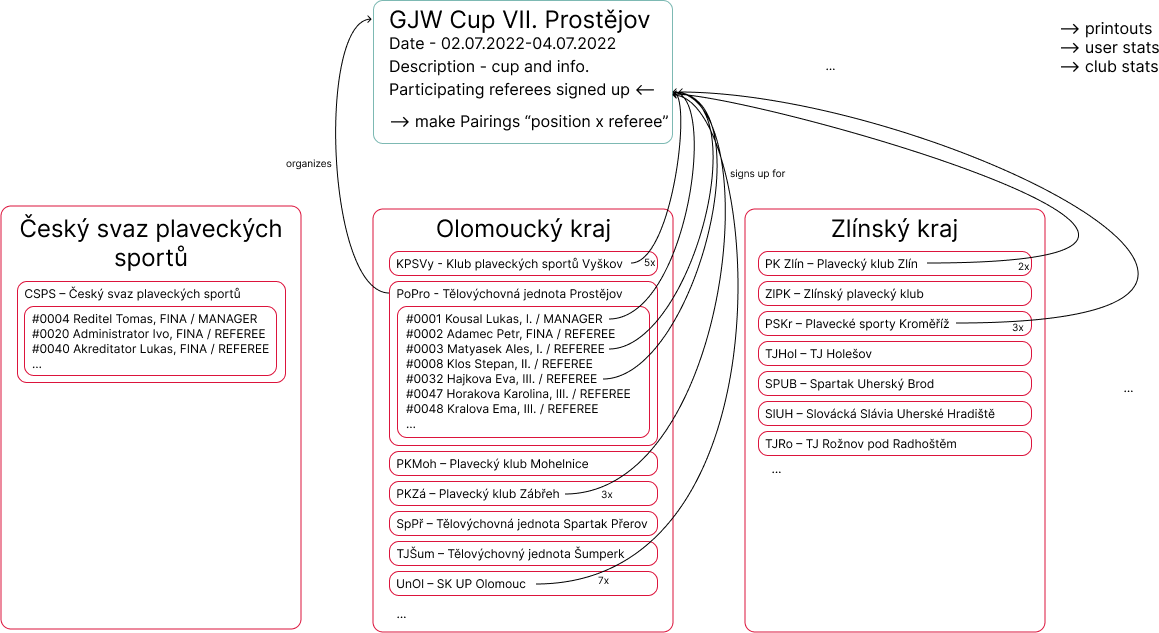
\includegraphics[scale=0.265]{img/swimmpair_schema.png}
  \caption{Preview of region-club-user grouping \& availability for the cup.}
  \label{fig1.1:grouping}
\end{figure}
The SwimmPair application should deliver public listing of all \textbf{users}, \textbf{cups}, \textbf{news}, \textbf{individual statistics} and \textbf{club statistics}. Application should allow to browse statistics on yearly basis. Structure (\autoref{fig1.1:grouping}) then has to be appropriately modeled as entities (\autoref{fig1.2:uml}). Proposition of entities-objects mappings (\autoref{fig2.6:enttousr} \autoref{fig2.7:entrels}) and database (\autoref{fig2.8:dbschemafull}) will be shown further down. 
%\newpage
\section{Stakeholders}
Groups direclty and indirectly interested in existence of this application and breakdown of its active/passive users.
\subsection*{Interest groups}
There are several entities that are interested in existence of this application. All these stakeholders will have their job facilitated and better organized to some extent thanks to existence of this application.
\newline
Interested stakeholders are:
\begin{itemize}
  \item \textbf{Czech Swimming Federation} - organization for competitive swimmers,
  \item \textbf{Olomouc Region}, \textbf{Zlin Region} - CSF regions administered together,
  \item \textbf{Lukas K.} from \textbf{TJ Prostejov} - coordinator who asked for this application.
\end{itemize}
\subsection*{Users of the application}
Users of our application will be Czech Swimming Federation members. If their \textbf{region} is \textbf{participating in this application}, clubs and referees belonging to this region must be in our system. Depending on their rank within the structure, individuals will be assigned one of these roles: 
\begin{itemize}
  \item \textbf{system administrator} ($\sim$1-3),
  \item \textbf{club manager} + also a swimming referee ($\sim$10s),
  \item \textbf{swimming referee} ($\sim$100s).
\end{itemize} 
Roles are self-descriptive. The coordinator (my friend), who came up with this idea for this application will be \textbf{system administrator} because he's been running all this agenda in Excel spreadsheets. \textbf{Club managers} are taking care of competitions on behalf of their club and \textbf{swimming referees} are common people who have some degree of knowledge about competitions and can participate as referees. \par 
The collected statistics will be used for accreditations granting, monitoring activity, and overall categorization.
\par
During the development process, we worked with two coordinators (who will also serve as system administrators) to iterate on the requirements and features for the application. \par
After the development was over, we performed test usability on \textbf{all three groups of users} via. SUS\footnote{\textbf{System Usability Scale} is a questionnaire to reveal how friendly a tested system is to target audience. We carried on initial testing for 20 people belonging to one of these 3 categories to find out if we met at least an average score which was determined to be 68/100.} questionnaire. We then version controlled, unit tested and CI pipelined \footnote{Brief overview of CI/CD pipelining \url{https://resources.github.com/ci-cd/} on GitHub.} our application. Despite advancements in automation, deployments are still performed manually.
%%%An~example citation: %\cite{Andel07}
\section{Functional requirements}
There are areas of similar tasks that we would like address and solve by our application by implementing features and ui pages for these purposes.
\subsection*{"C" as Cup administration}
\begin{enumerate}
    \item \lbrack club manager\rbrack \,needs to\, \lbrack create swimming cup\rbrack \,in order to\, \lbrack publish cup and invite others to participate\rbrack
    \item \lbrack club manager\rbrack \,needs to\, \lbrack create pairing for swimming cup\rbrack \,in order to\, \lbrack finalize preparations of the cup the day before it takes place\rbrack
    \item \lbrack club manager\rbrack \,needs to\, \lbrack preview cups and print pairing\rbrack \,in order to\, \lbrack perform inspection and publish information offline\rbrack
    \item \lbrack club manager\rbrack \,needs to\, \lbrack participate in cup or participate with teammates\rbrack \, in order to\, \lbrack help swimming cup to take place\rbrack
\end{enumerate} 
\subsection*{"R" as Referees administration \& overview}
\begin{enumerate}
\item \lbrack club manager\rbrack \,needs to\, \lbrack manage swimming club\rbrack \,in order to\, \lbrack keep information and users up to date\rbrack
\item \lbrack club manager\rbrack \,needs to\, \lbrack perform referees managment\rbrack \, in order to \, \lbrack keep referees up to date\rbrack
\item \lbrack referee\rbrack \,needs to\, \lbrack view statistics of referees\rbrack \, in order to \, \lbrack have track record about personal participation\rbrack
\item \lbrack club manager\rbrack \,needs to\, \lbrack view statistics of clubs\rbrack \, in order to \, \lbrack have information about performance within one's own club\rbrack
\item \lbrack club manager\rbrack \,needs to\, \lbrack perform club managment\rbrack \, in order to \, \lbrack keep own club up to date\rbrack
\item \lbrack system administrator\rbrack \,needs to\, \lbrack manage referees\rbrack \, in order to \, \lbrack add, remove, update users in the dataset\rbrack
\item \lbrack system administrator\rbrack \,needs to\, \lbrack list referees overview\rbrack \, in order to \, \lbrack see activity of referees\rbrack
\end{enumerate} 
\subsection*{"S" as Stakeholders interests}
\begin{enumerate}
  \item \lbrack system administrator\rbrack \,needs to\, \lbrack have overview of clubs\rbrack \, in order to \, \lbrack be informed about various things\rbrack
  \item \lbrack stakeholder\rbrack \,needs to\, \lbrack have overall categorization of federation\rbrack \, in order to \, \lbrack use application for administrative purposes\rbrack
  \item \lbrack stakeholder\rbrack \,needs to\, \lbrack have database archivation of federation\rbrack \, in order to \, \lbrack use application as an archivation tool\rbrack
  \item \lbrack stakeholder\rbrack \,needs to\, \lbrack have information about participations\rbrack \, in order to\, \lbrack grant accreditations to referees for next season\rbrack
  \item \lbrack system administrator\rbrack \,needs to\, \lbrack publish news\rbrack \, in order to \, \lbrack notify everybody about important whereabouts\rbrack
  \item \lbrack system administrator\rbrack \,needs to\, \lbrack edit page/s\rbrack \, in order to \, \lbrack change static public info in the application\rbrack
\end{enumerate}
\section{Domain model}
Let's look at the entities which have to be represented in our system one by one - starting from the most important ones. We will outlay entities and their relations. After basic idea of entities and their relations is established we proceed to project specification to delve further into the implementation details. Our approach was, however, more iterative - this retrospective domain model represents only a snapshot of the implementation details that we were specifying throughout our development process.
\par
\subsection*{Cup}
\textbf{Cup is the most important entity.} A swimming \textbf{cup} contains name, description, date and is affiliated to organizing club. Cup serves two purposes. \textbf{Firstly}, referees assignment for specific tasks (time tracking, computer support, main organizer, etc.) has to be \textbf{ready by the time the event takes place}. \textbf{Secondly}, statistics summing up participations of referees and clubs have to be calculated for each year from all cups in this time period. We also have to discriminate between upcoming and already past cups. Upcoming cups should be displayed, past cups should reside in archive to be revisited for statistical purposes.
\iffalse\subsection*{User - strike}
\par
User is an entity modelling swimming referee. A referee participating in this system falls in one of three categories. These categories or levels if you wish are \textbf{referee}, \textbf{club manager} and \textbf{system administrator}. User has to be uniquely identifiable. A person i.e. User in the system is going to have profile information such as first name, family name, email address. Good practice of using email address as a login information is going to be used here. User must also contain SwimmPair hierarchy listed above\footnote{\textbf{Rights} - referee 0 / club manager 1 / system administrator 2} and indicator of one's skill and knowledge in the swimming field, i.e. referee category. User must also belong to exactly one club in our system.
\fi
\subsection*{Referee}
Referee is a person and a main workforce during swimming cup. A referee is a member of club who participates on the club's behalf in cups. A referee's level of expertise is described by one of the several ranks\footnote{\textbf{Referee Rank} - 1/2/3/4/FINA at \url{https://www.czechswimming.cz/index.php/rozhodci}}. Referee is assigned to one or more Positions, such as \textbf{Timekeeping} or \textbf{PC Support} and is in charge of the task for duration of the cup. 
\subsection*{Club manager}
Club manager is usually one person who is in charge of club administration. Club manager organizes cup on behalf of club and acts as a main figure during it. Club managers may also assist with certain tasks, but their role is primarily administrative. The club manager is responsible for pairing referees with suitable positions and creating work schedules for all participants.
\subsection*{Coordinator}
The coordinator is the head of swimming in a specific region. They prepare budgets, plan tournaments and manage the administration and database of referees, clubs, and cups. They are the most important person in the administrative hierarchy of swimming.
\subsection*{Club}
\par
A club is an administrative unit that groups people together in the same city. The club has a specific name, abbreviation, and id in the Czech Swimming Federation, and a club logo can be included as well. The club serves as the formal authority organizing the cup by a user who is the club manager. The club is affiliated to the region. Performance statistics of members of the club at swimming competitions must be implemented. These statistics have an informative character and will save time compared to the current status quo of keeping track of presence and work descriptions in Excel spreadsheets.
\subsection*{Region}
There are 13 regions in the Czech Republic, and we are currently addressing this problem for two regions that are being administered together. Other regions may also choose to join. Each club is located in one of these regions. When a new club starts using SwimmPair in the future, a new region will need to be added and potential clubs created and attached to this region.
\iffalse
\subsection*{Availability}
Referee is available in the time of Cup.
\fi

\subsection*{Pairing}
Pairing is simple list of pairs (\textbf{position} x \textbf{referee}) $\rightarrow$ \textbf{cup}.
\subsection*{Position}
Predefined list of tasks necessary to be taken care of at each cup. This list is probably never going to change since there is a fixed set of roles. Referees are going to be assigned to these positions for each cup.
\newpage
\subsection*{Schema of entities and their connections}
Majority of focus should be on \textbf{referee}, \textbf{club manager} and \textbf{cup} in the presented schema(\autoref{fig1.2:uml}). Referees belong to clubs which belong to regions. These two entities \textbf{referee} and \textbf{cup} along with \textbf{position} will then be brought together as \textbf{pairing} which contains referees that are available for specific cups and will be performing work at a specified position. Referees must be available in specific time but \textbf{pairing} is where each record can be assigned a position from prescripted \textbf{positions}.
\begin{figure}[h]
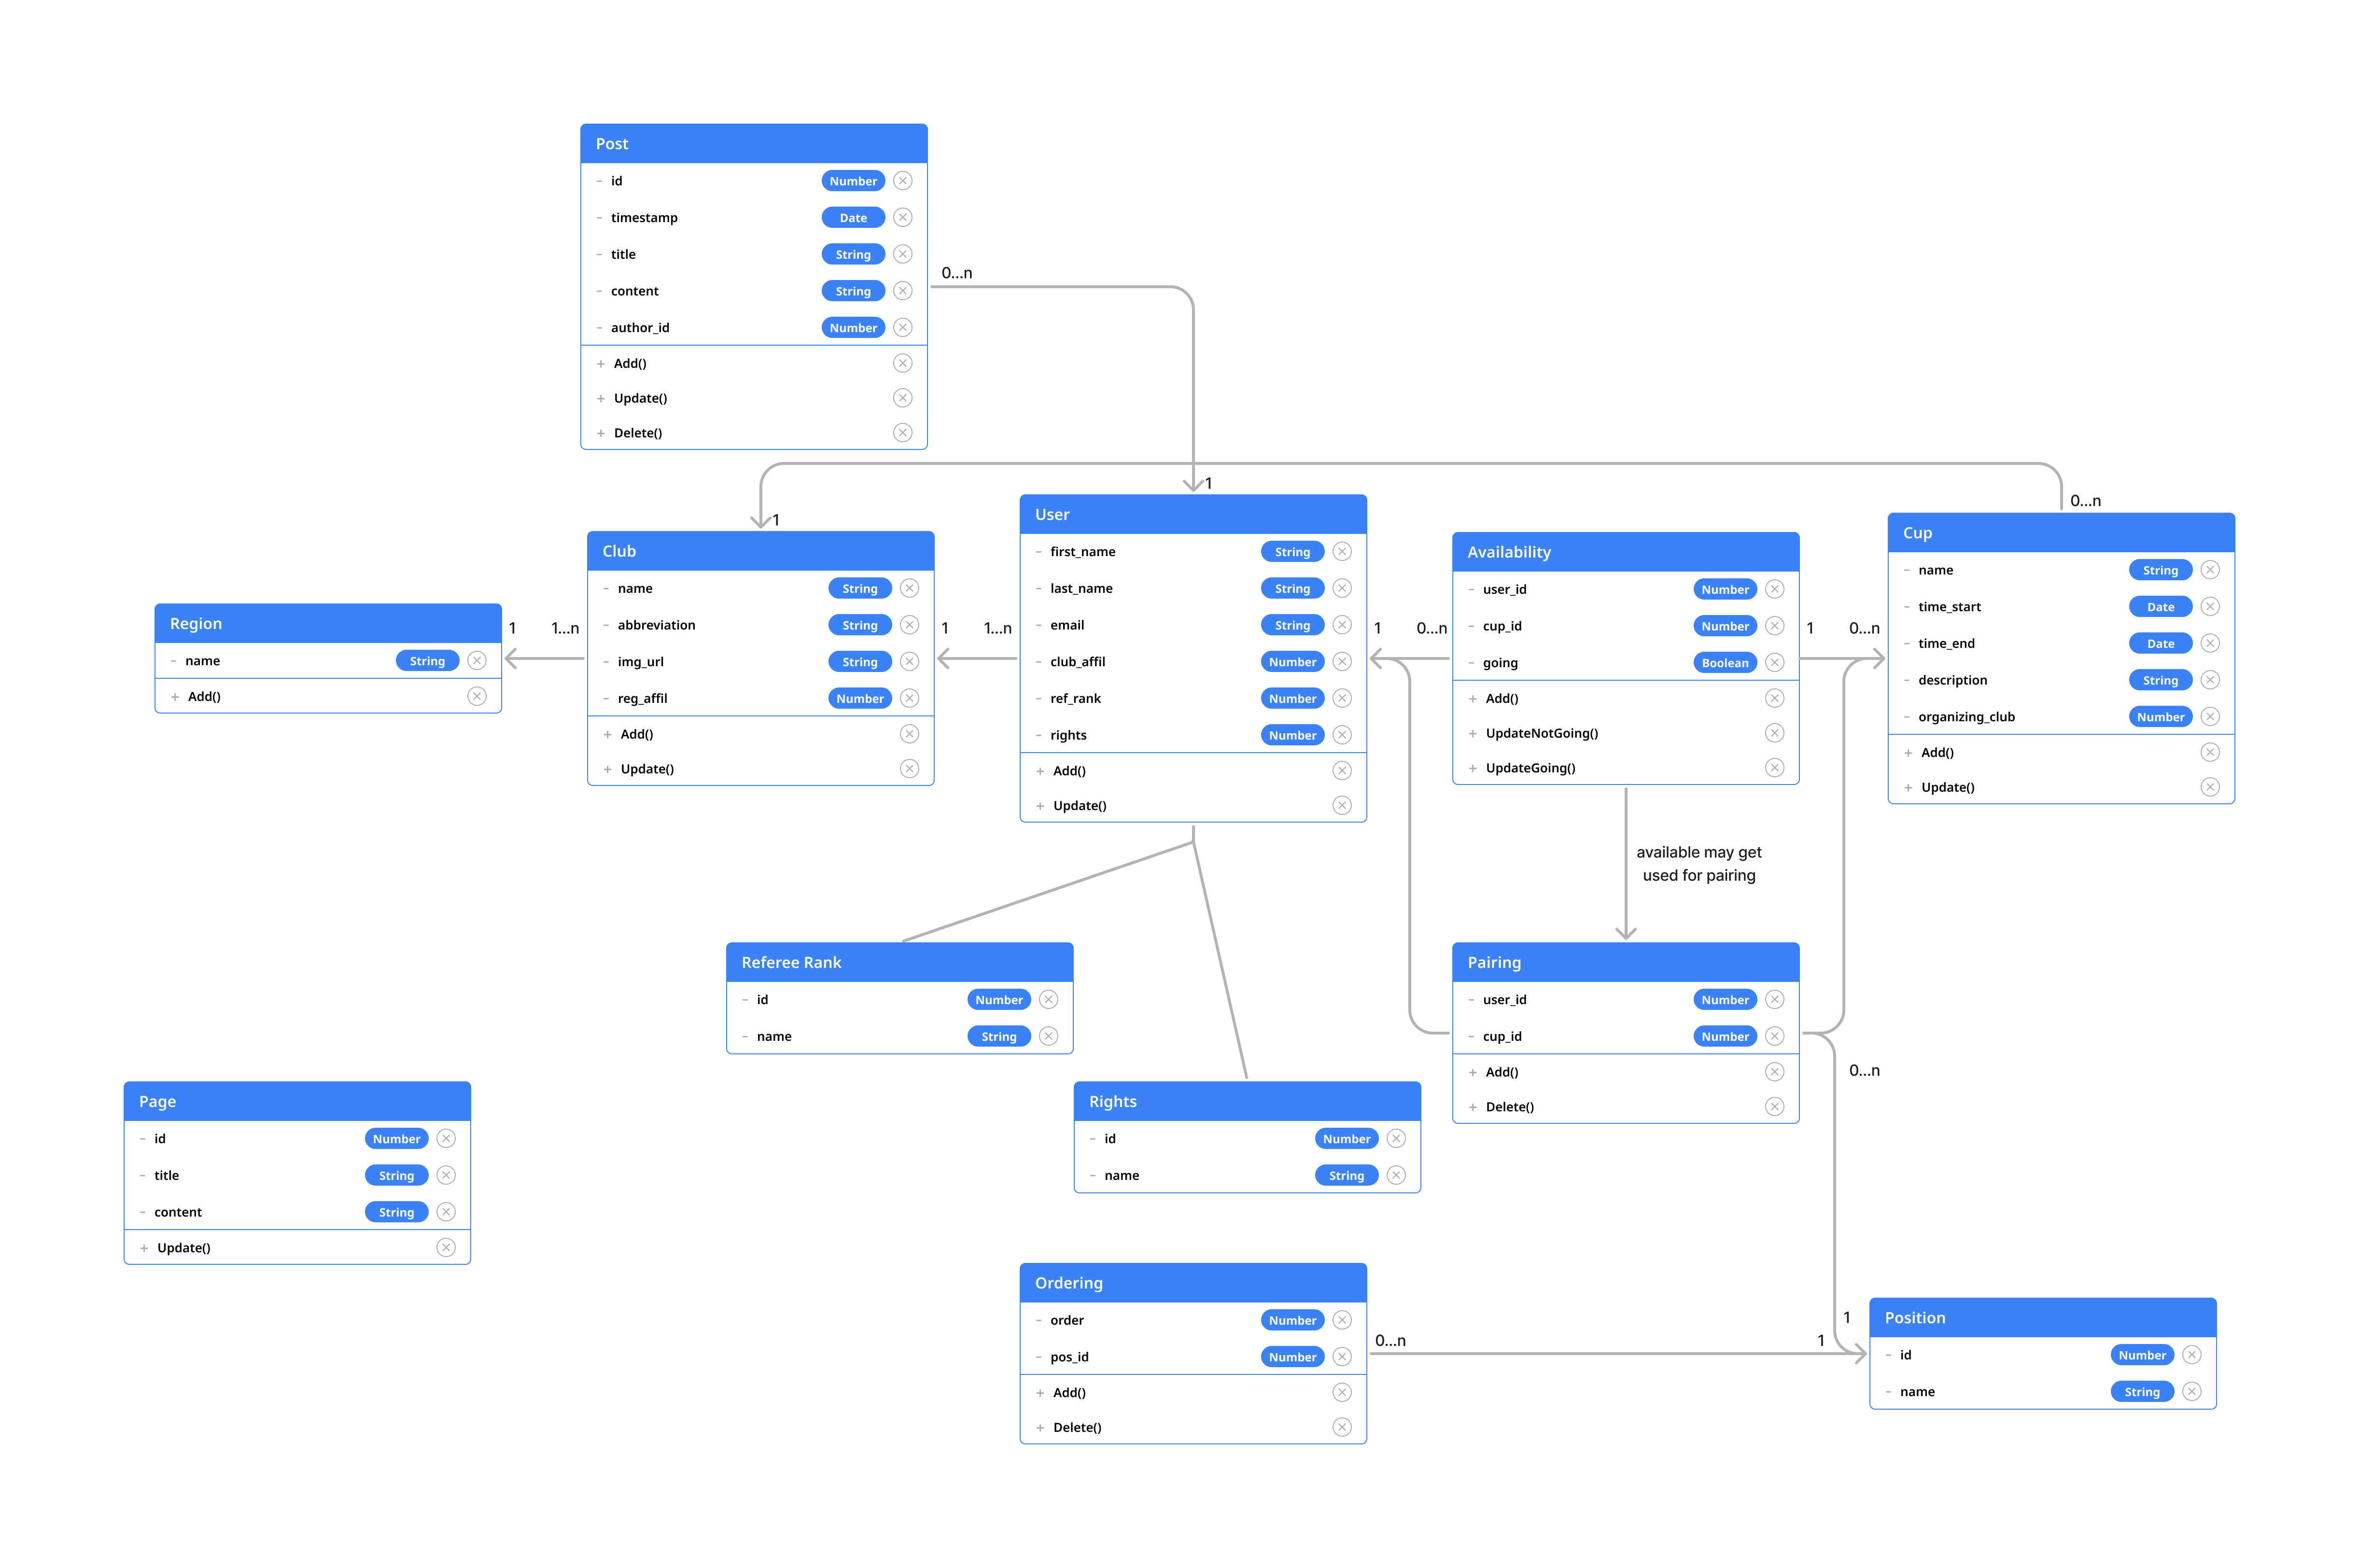
\includegraphics[scale=0.160]{img/swimmpair_uml.png}
  \caption{UML Class Diagram outlaying the administrative structure.}
  \label{fig1.2:uml}
\end{figure}

\section{Quality/Usability Requirements}
Several good practices have to be implemented to make SwimmPair easy to use. Although some of these practices are well-known and others are situation-specific, they all share a common goal: to improve the usability of the application.
\subsection*{Smooth frontend browsing}
To make SwimmPair user-friendly, the frontend should be designed to be easy to use. This includes reducing page reloads, which can be achieved through asynchronous JavaScript calls to obtain partial data. The obtained data can then be used to modify the DOM using the appropriate functions. 
\subsection*{Multiple device types}
It is certain that there are users who want to browse our application on a PC, tablet, or smartphone so a responsive design is a necessity. CSS3 supports media queries\footnote{\url{https://developer.mozilla.org/en-US/docs/Web/CSS/Media_Queries}}, which we will use to create device-specific styling.
\subsection*{Assigning referees to positions via. drag'n'drop}
Assigning referees to positions for cups should be implemented via drag'n'drop. Dragging a referee, moving referee over the region specified for the positions and releasing mouse button. Double clicking this person is a good way of removing it.
\subsection*{Printouts of pairing}
Upcoming cup can be directly printed\footnote{\url{https://developer.mozilla.org/en-US/docs/Web/CSS/Media_Queries/Using_media_queries\#targeting_media_types}} from website and hanged as data printout. 
%\subsection*{Mobile administration}
%Since some things could be done from phone, a phone app without a necessity of web browser will have more native feel. Assigning by drag and drop would be very %hazardeous to do with regards to difference between mouse and finger. Also we are not certain that the Events are the same. Therefore full version %adminsitrative app should be necessary to be provided.
\subsection*{Appropriate design}
Red, blue, and gray are common colors found at swimming pools, and they will be used in our system's design. Our UI elements should have a fresh, lightweight look that doesn't feel heavy or overwhelming to users. Specifically, we'll use these colors to create an interface that's easy to navigate and visually appealing. For example, we might use blue to highlight important information, or red to indicate errors or warnings. By using these colors consistently throughout the system, we can create a cohesive and user-friendly experience for our users.
\section{Scalability/Usability Requirements}
Application is initially going to be used for 2 regions and approximately 100 referees. Maximum saturiation would mean that system is used in the whole Czech Republic. Maximum traffic is then 5-6x larger load than the current one.
\newline
\par
\textbf{Potentially looming issues:}
\begin{itemize}
  \item \textbf{performance issues} - shouldn't be problem using LAMP stack, 
  \item \textbf{larger traffic} - can be solved via Kubernetes autoscaling \footnote{\url{https://kubernetes.io/docs/tasks/run-application/horizontal-pod-autoscale/}},  
  \item \textbf{simulaneous application edits} - can be solved by locking and comparing hashes of states before comitting changes to database,
  \item \textbf{sessions consistency} - can be solved (even throughout cluster restart) using Redis\footnote{\url{https://redis.io}} for (persistent) session handling.
\end{itemize}
These issues can be easily tackled if they are kept in mind during the development.